\subsection{Secciones de la aplicación.}

\subsubsection{Pantalla de inicio (Home).}

La primera interfaz que el usuario encuentra al iniciar el launcher es la vista de tareas y hábitos. Desde aquí el usuario podrá crear, editar, completar y eliminar, así como también acceder al histórico de los elementos mencionados. La lista está encabezada por los hábitos creados, que se muestran solo si el día actual está entre los días de la semana seleccionados para su repetición; le siguen las tareas, ordenadas automáticamente según su fecha de creación, vencimiento y prioridad asignadas.

\begin{figure}[ht]
  \centering
  \captionsetup{justification=centering}
  \begin{minipage}{0.43\textwidth}
    \caption{Home: Vista de tareas y hábitos.}
    \label{fig:home:vista_tareas_habitos}
    \centering
    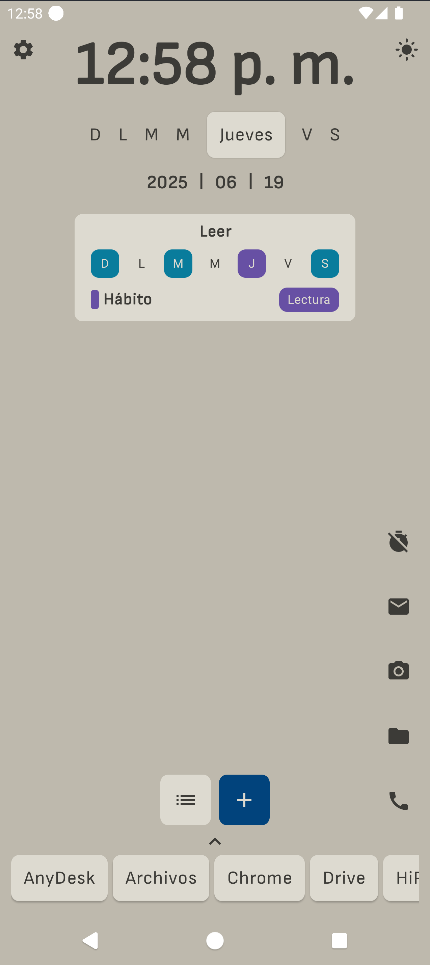
\includegraphics[width=\textwidth]{Figuras/secciones/home_1.png}
  \end{minipage}\hspace{0.05\textwidth}
  \begin{minipage}{0.43\textwidth}
    \caption{Home: Crear tarea o hábito.}
    \label{fig:home:crear_tarea_habito}
    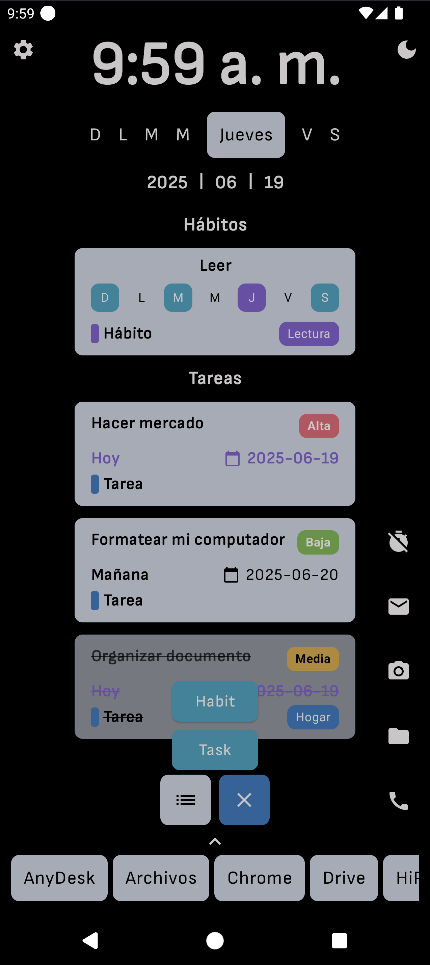
\includegraphics[width=\textwidth]{Figuras/secciones/home_2.png}
    \centering
  \end{minipage}
\end{figure}

Al crear un hábito (ver Figura \ref{fig:home:crear_habito}) o una tarea (ver Figura \ref{fig:home:crear_tarea}), se mostrará una ventana modal con un pequeño formulario para especificar sus propiedades. Sus diferencias radican en que en el caso del hábito, se podrán seleccionar los días de la semana que se mostrará en la lista y, de asignarse una fecha de fin, se dejará de mostrar posterior a esta. En el caso de la tarea, de asignarse una fecha límite, se mostrará cuántos días faltan y se marcará como atrasada si no se cumple en el plazo establecido. En ambos casos, se podrá crear una categoría directamente en el modal o seleccionar una ya existente. Al guardar el elemento, se notifica al ViewModel correspndiente mediante un \textit{Event}, quien envía la información al UseCase y actualiza la base de datos, reflejando la tarea o hábito recién creado gracias a las funciones de data binding que ofrecen los \textit{Flows} \cite{Flows} en Kotlin.

\begin{figure}[ht]
  \centering
  \captionsetup{justification=centering}
  \begin{minipage}{0.43\textwidth}
    \caption{Home: Crear hábito.}
    \label{fig:home:crear_habito}
    \centering
    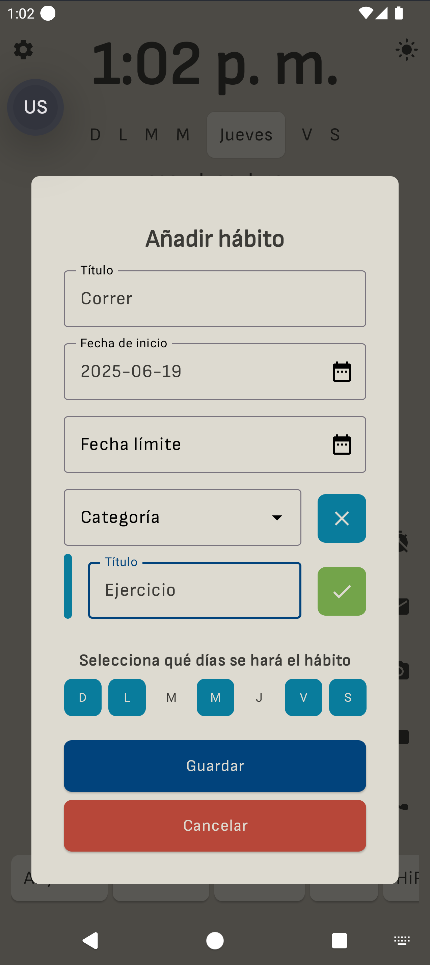
\includegraphics[width=\textwidth]{Figuras/secciones/crear_habito.png}
  \end{minipage}\hspace{0.05\textwidth}
  \begin{minipage}{0.43\textwidth}
    \caption{Home: Crear tarea.}
    \label{fig:home:crear_tarea}
    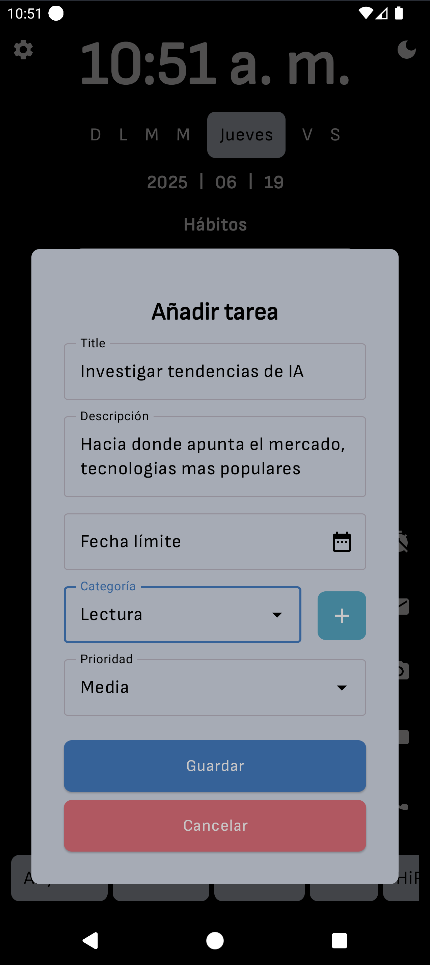
\includegraphics[width=\textwidth]{Figuras/secciones/crear_tarea.png}
    \centering
  \end{minipage}
\end{figure}

Los widgets de hora y fecha también tienen un papel importante en esta pantalla, haciendo consciente al usuario, de manera constante, del momento en el que se encuentra. Al tocar sobre estos widgets, se puede acceder a las aplicaciones de reloj y calendario predeterminadas del smartphone. La interfaz también incorpora una barra de aplicaciones esenciales, en la parte inferior del costado derecho, que el usuario puede configurar para mostrar u ocultar según sus preferencias, proporcionando acceso inmediato a las aplicaciones de \textbf{teléfono, archivos, cámara, correo y la función de límite de tiempo de las aplicaciones}, dando un extra de utilidad sin perder su enfoque minimalista.

Del lado izquierdo de la vista de tareas y hábitos, se encuentra la implementación de la técnica de gestión del tiempo más conocida en el mundo de la productividad: Pomodoro. Esta técnica consiste en dividir el tiempo en intervalos de, generalmente, 25 minutos de trabajo seguidos de un descanso de 5 minutos. La idea de implementar una técnica de gestión del tiempo en el launcher es que el usuario pueda concentrarse en una tarea específica durante un período determinado. Al iniciar el temporizador, comenzará a contar el tiempo del ciclo establecido en el tiempo de sesión. Al finalizar, se le notificará al usuario mediante un sonido para que tome un breve descanso. La Figura \ref{fig:pomodoro:tiempo_trabajo} y la Figura \ref{fig:pomodoro:tiempo_descanso} muestran el temporizador de Pomodoro en funcionamiento.

\begin{figure}[ht!]
  \centering
  \captionsetup{justification=centering}
  \begin{minipage}{0.43\textwidth}
    \caption{Pomodoro: Tiempo de trabajo.}
    \label{fig:pomodoro:tiempo_trabajo}
    \centering
    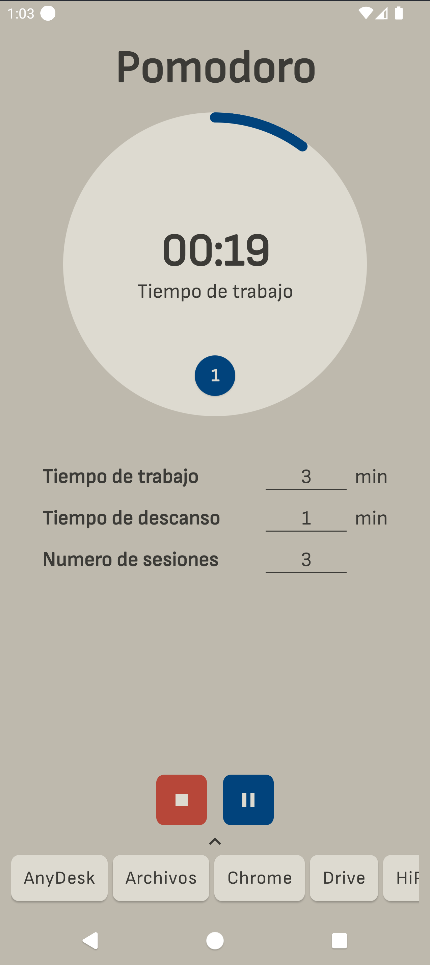
\includegraphics[width=\textwidth]{Figuras/secciones/pomodoro_tiempo_trabajo.png}
  \end{minipage}\hspace{0.05\textwidth}
  \begin{minipage}{0.43\textwidth}
    \caption{Pomodoro: Tiempo de descanso.}
    \label{fig:pomodoro:tiempo_descanso}
    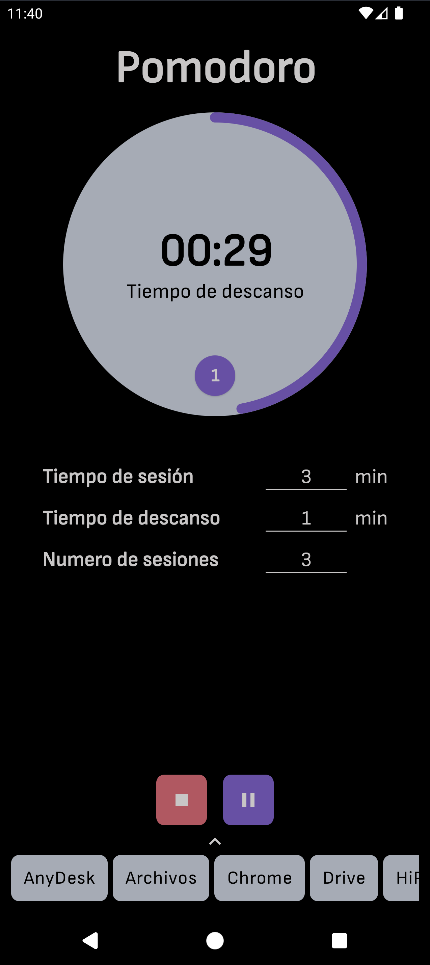
\includegraphics[width=\textwidth]{Figuras/secciones/pomodoro_tiempo_descanso.png}
    \centering
  \end{minipage}
\end{figure}

\subsubsection{Menú de aplicaciones.}

El menú de aplicaciones es una de las secciones más importantes del launcher, ya que permite al usuario acceder a todas las aplicaciones instaladas en su dispositivo. Sin duda es la sección que, a nivel visual, más difiere con respecto a los launchers tradicionales, ya que no muestra los íconos de las aplicaciones, solo una lista con los nombres de las aplicaciones, organizadas alfabéticamente. La intención es que el usuario sepa claramente qué aplicación está a punto de abrir, sin ser influenciado inconscientemente por el diseño llamativo de los íconos de las aplicaciones. 

Se divide en dos secciones principales: la \textbf{barra de búsqueda} y la \textbf{lista de aplicaciones}. En la lista de aplicaciones, el usuario puede desplazarse verticalmente para buscar la que desea usar. Al tocar en una de ellas, se abrirá la aplicación correspondiente. Al dar una pulsación sostenida, se harán visibles tres (3) opciones: \textbf{Fijar a la pantalla de inicio, información de la aplicación y desinstalar}. Aquellas aplicaciones fijadas se mostrarán en la parte inferior de la sección de home para un acceso más inmediato. La barra de búsqueda permite al usuario encontrar aplicaciones con más precisión: A medida que el usuario escribe, la lista de aplicaciones se filtra en tiempo real, mostrando solo aquellas que coinciden con el texto ingresado. También se mostrará, en la última posición, un botón en la lista de aplicaciones para buscar el texto ingresado en la Web, abriendo el navegador predeterminado del dispositivo.

Este comportamiento se logra mediante el uso de la API de \texttt{PackageManager} en Android, la cual proporciona la información de las aplicaciones instaladas; y la declaración de acciones e intercambio de información a través de \texttt{Intents}. Los Intents expresan lo que una aplicación desea enviar o realizar, y permiten al launcher interactuar con el sistema operativo para abrir aplicaciones, diálogos del sistema o realizar búsquedas en la Web. La lista de aplicaciones se guarda en la base de datos de Room al iniciar el launcher por primera vez, y se actualiza cada vez que el sistema envía un \texttt{Broadcast} para notificar un cambio en las aplicaciones instaladas. A su vez, el launcher recibe ese Broadcast mediante un \texttt{BroadcastReceiver}, que escucha específicamente Intents de tipo \texttt{ACTION\_PACKAGE\_ADDED} o \texttt{ACTION\_PACKAGE\_REMOVED}. La implementación del menú se muestra en la Figura \ref{fig:menu_lista_aplicaciones} y la Figura \ref{fig:menu_busqueda_aplicaciones}.

\pagebreak

\begin{figure}[ht!]
  \centering
  \captionsetup{justification=centering}
  \begin{minipage}{0.43\textwidth}
    \caption{Menú: Lista de aplicaciones.}
    \label{fig:menu_lista_aplicaciones}
    \centering
    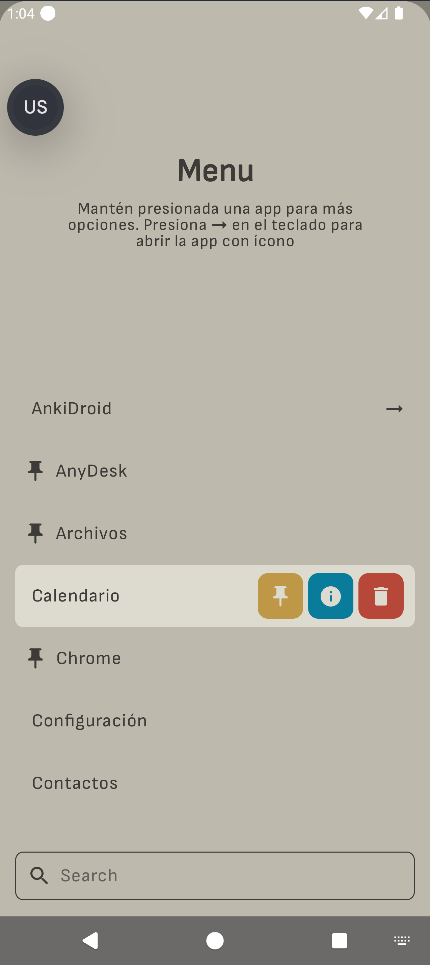
\includegraphics[width=\textwidth]{Figuras/secciones/menu_lista_aplicaciones.png}
  \end{minipage}\hspace{0.05\textwidth}
  \begin{minipage}{0.43\textwidth}
    \caption{Menú: Búsqueda de aplicaciones.}
    \label{fig:menu_busqueda_aplicaciones}
    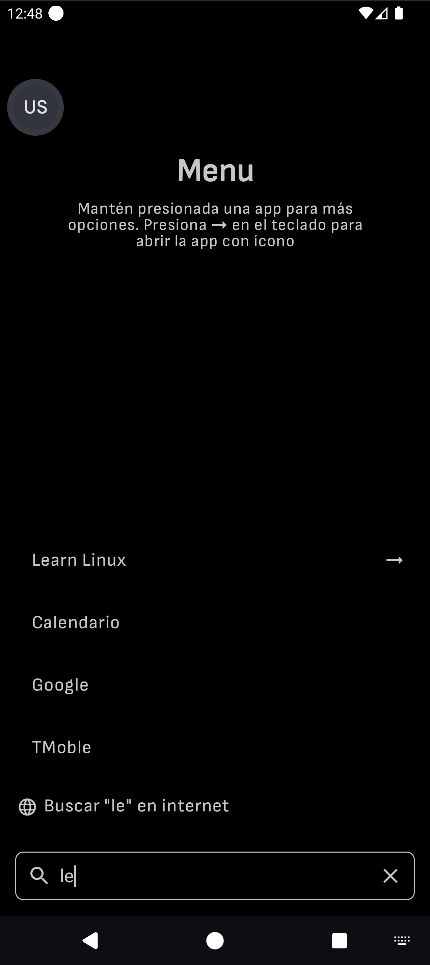
\includegraphics[width=\textwidth]{Figuras/secciones/menu_busqueda_aplicaciones.png}
    \centering
  \end{minipage}
\end{figure}

\subsubsection{Ajustes y personalización.}

La sección de ajustes, accedida desde el engranaje de la sección de home en la esquina superior izquierda (ver Figura \ref{fig:home:vista_tareas_habitos} y Figura \ref{fig:home:crear_tarea_habito}), permite al usuario personalizar ligeramente su experiencia de uso dentro del launcher. Cuenta con las siguientes opciones:

\begin{itemize}
\item Fondo de pantalla de color sólido - Opción activada
\item Abrir teclado automáticamente en el menú de aplicaciones
\item Mostrar "buscar en internet" en el menú de aplicaciones
\item Motor de búsqueda
\item Mostrar atajos esenciales
\item Establecer Dino como Launcher predeterminado
\end{itemize}

Así mismo, en la sección de home, al lado opuesto del engranaje se encuentra el ícono para el cambio de tema, que cuenta con tres (3) modos: \textbf{Claro}, \textbf{oscuro} y \textbf{automático} (predeterminado del sistema). Las variantes del tema ya se han podido evidenciar a lo largo de este capítulo, y se implementaron utilizando el sistema de temas de Jetpack Compose, consignando los colores, tipografías y estilos definidos en el proceso de diseño de los mockups.

\begin{figure}[ht!]
  \centering
  \captionsetup{justification=centering}
    \caption{Ajustes.}
    \label{fig:ajustes}
    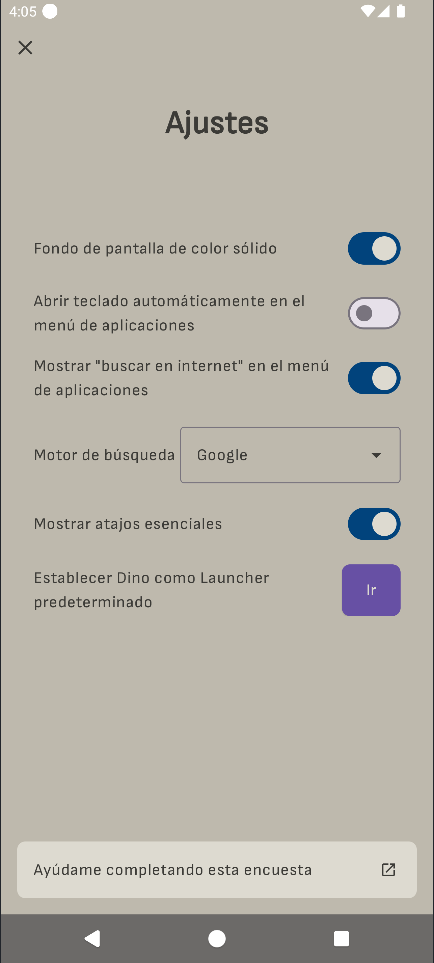
\includegraphics[width=0.43\textwidth]{Figuras/secciones/ajustes.png}
    \centering
\end{figure}


\subsubsection{Límite de tiempo de aplicaciones.}

Otro pilar fundamental del launcher es la funcionalidad de límite de tiempo de aplicaciones, que permite al usuario establecer restricciones en el uso diario de aplicaciones específicas. Para acceder a la funcionalidad, el usuario debe tocar el ícono de bloqueo de tiempo presente en la barra de aplicaciones esenciales del home, como se puede ver en la Figura \ref{fig:home:vista_tareas_habitos} y la Figura \ref{fig:home:crear_tarea_habito}, y aceptar dos (2) permisos adicionales: \textbf{Acceso a estadísticas de uso} y \textbf{mostrar sobre otras aplicaciones}, requeridos por el launcher para que esta característica funcione correctamente. Al navegar a esta sección, aparecerá una lista de las aplicaciones limitadas y el tiempo en minutos que el usuario las ha utilizado en el día actual, mostrado en la Figura \ref{fig:limite_tiempo_aplicaciones}. Para limitar una aplicación, basta con ir a seleccionar aplicaciones, mostrado en la Figura \ref{fig:seleccionar_aplicaciones_limite_tiempo}, y fijar un tiempo máximo de uso.


\begin{figure}[ht!]
  \centering
  \captionsetup{justification=centering}
  \begin{minipage}{0.43\textwidth}
    \caption{Límite de tiempo: Uso del día actual.}
    \label{fig:limite_tiempo_aplicaciones}
    \centering
    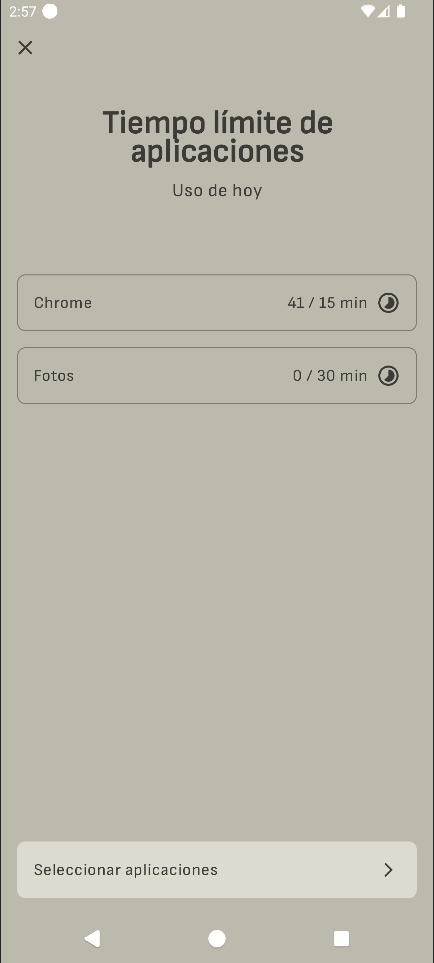
\includegraphics[width=\textwidth]{Figuras/secciones/limite_tiempo_aplicaciones.png}
  \end{minipage}\hspace{0.05\textwidth}
  \begin{minipage}{0.43\textwidth}
    \caption{Límite de tiempo: Selección de aplicaciones.}
    \label{fig:seleccionar_aplicaciones_limite_tiempo}
    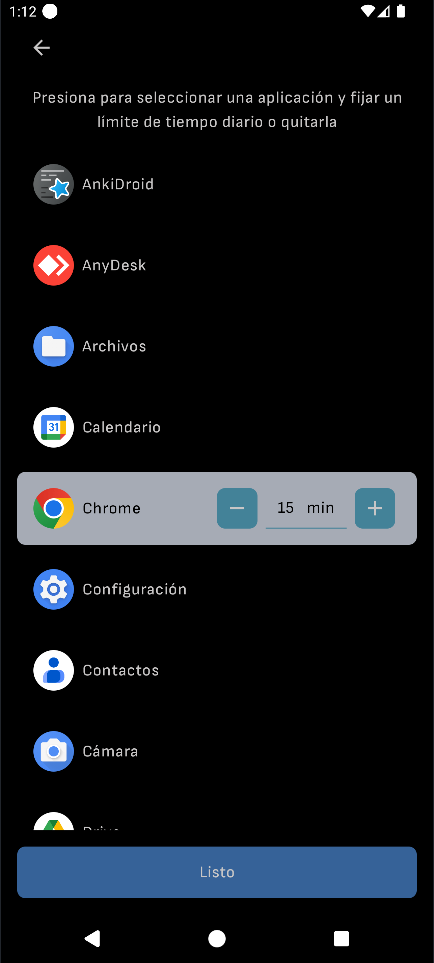
\includegraphics[width=\textwidth]{Figuras/secciones/seleccionar_aplicaciones_limite_tiempo.png}
    \centering
  \end{minipage}
\end{figure}

A través de la API de \texttt{UsageStatsManager}, el launcher obtiene las estadísticas de uso de las aplicaciones instaladas y, si hay alguna que se encuentre limitada desde el launcher, muestra su información del tiempo de uso. Aceptar los permisos ya mencionados inicia un tipo de serivicio llamado \texttt{Foreground Service}, el cual se encarga de monitorear el uso de las aplicaciones cada minuto y actualizar la interfaz del launcher o los campos que habilitan el bloqueo a las aplicaciones limitadas si el tiempo establecido ya se cumplió. A diferencia de los servicios normales, un Foreground Service muestra una notificación persistente al usuario para hacerle saber de su ejecución (ver Figura \ref{fig:foreground_service}) y el sistema tiene predilección por mantenerlo activo. Al llegar al límite de tiempo en alguna aplicación limitada, el launcher mostrará una interfaz notificando al usuario e invitándolo a abandonar la aplicación por el día de hoy. Esta interfaz se muestra en la Figura \ref{fig:limite_tiempo_alcanzado}.

\begin{figure}[ht!]
  \centering
  \captionsetup{justification=centering}
    \begin{minipage}{0.43\textwidth}
    \caption{Límite de tiempo alcanzado.}
    \label{fig:limite_tiempo_alcanzado}
    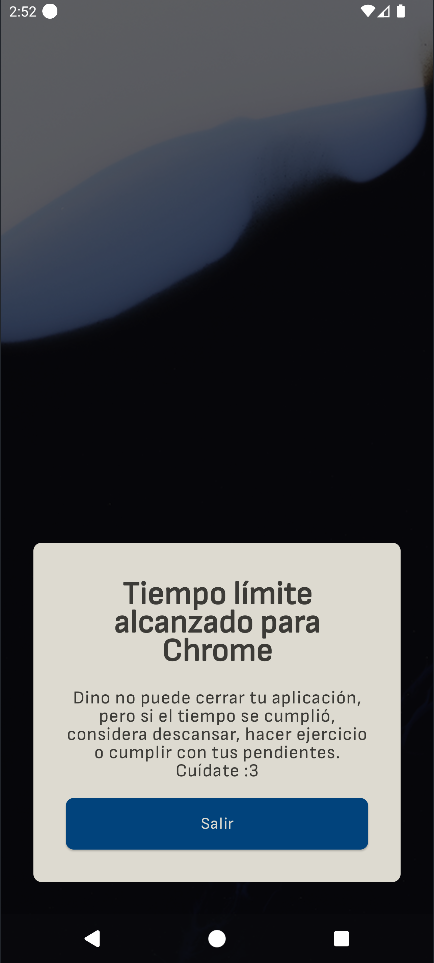
\includegraphics[width=\textwidth]{Figuras/secciones/limite_tiempo_alcanzado.png}
    \centering
  \end{minipage}\hspace{0.05\textwidth}
  \begin{minipage}{0.43\textwidth}
    \caption{Notificación del Foreground Service.}
    \label{fig:foreground_service}
    \centering
    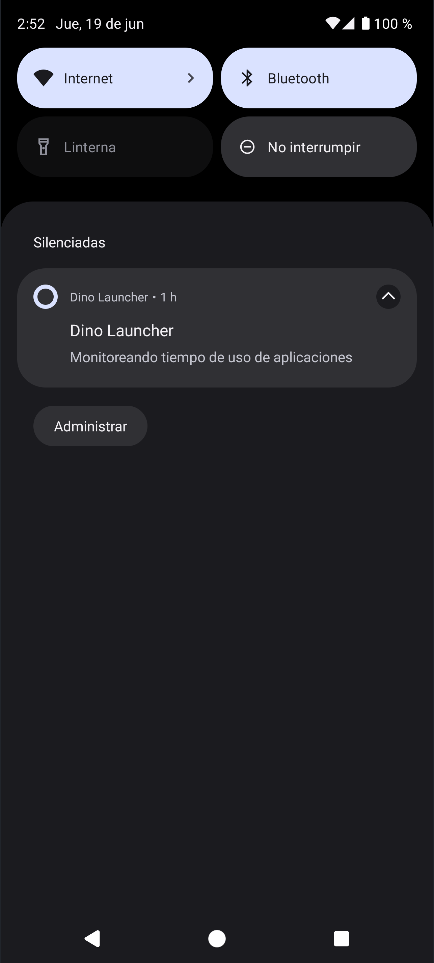
\includegraphics[width=\textwidth]{Figuras/secciones/foreground_service.png}
  \end{minipage}
\end{figure}

\subsection{Limitaciones.}

Es importante señalar que, aunque el servicio de monitoreo implementado en el launcher verifica el uso de aplicaciones cada minuto mediante la API de UsageStatsManager, el sistema operativo Android no actualiza las estadísticas de uso con la misma frecuencia. Esta diferencia temporal puede ocasionar que la interfaz de límite de tiempo alcanzado aparezca varios minutos después de que efectivamente se haya superado el umbral establecido, afectando la efectividad del enfoque restrictivo. 

Adicionalmente, debido a las restricciones de seguridad en Android, el launcher no posee la capacidad de controlar directamente la actividad de otras aplicaciones una vez que han sido iniciadas. Por esto, el launcher no puede forzar el cierre automático de aplicaciones cuando se cumple el límite de tiempo establecido, ni tampoco puede impedir que estas sean accedidas a través de mecanismos alternativos del sistema, tales como la pantalla de aplicaciones recientes, notificaciones entrantes, enlaces desde otras aplicaciones o si estas son iniciadas por el propio sistema operativo.